\subsection{Cadeia de Markov com $m$ estados}

\begin{questions}
\question{
Considere a cadeia de Markov com $m$ estados ilustrada abaixo, onde todas as transições possuem a mesma probabilidade.

\begin{figure}[h]
\centering
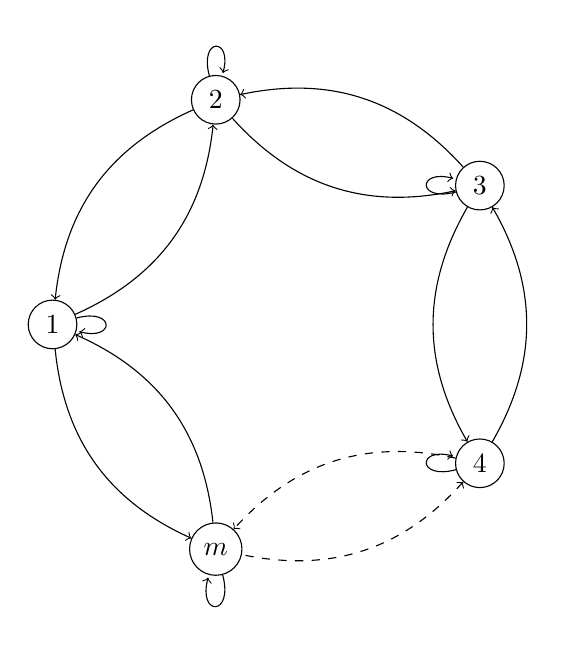
\begin{tikzpicture}

\def \n {5}
\def \radius {3cm}
\def \margin {8} % margin in angles, depends on the radius
\def \m {0}
\pgfmathtruncatemacro\m{\n-2}
\foreach \s in {1,...,\m} {
  \node[draw, circle] (\s) at ({360/\n*(1-\s)}:-\radius) {$\s$};
}

\def \s {0}
\pgfmathtruncatemacro\s{\n-1}
\node[draw, circle] (\s) at ({360/\n*(1-\s)}:-\radius) {$\s$};

\pgfmathtruncatemacro\s{\s+1}
\node[draw, circle] (\s) at ({360/\n*(1-\s)}:-\radius) {$m$};

\path
(1) edge[loop right]  node{}  (1)
(2) edge[loop above]  node{}  (2)
(3) edge[loop left]  node{}  (3)
(4) edge[loop left]  node{}  (4)
(5) edge[loop below]  node{}  (5)

(1) edge[->, bend right]  node{}  (2)
(1) edge[<-, bend left]  node{}   (2)
(2) edge[->, bend right]  node{}  (3)
(2) edge[<-, bend left]  node{}   (3)
(3) edge[->, bend right]  node{}  (4)
(3) edge[<-, bend left]  node{}   (4)
(4) edge[dashed, ->, bend right]  node{}  (5)
(4) edge[dashed, <-, bend left]  node{}   (5)
(5) edge[->, bend right]  node{}  (1)
(5) edge[<-, bend left]  node{}   (1)
;

\end{tikzpicture}
\end{figure}

\begin{parts}
\part
Determine a distribuição de estado estacionário.

\part 
Determine a taxa de entropia desta cadeia de Markov.

\end{parts}

}


\begin{solution}
\begin{parts}
\part
\begin{verbatim}
pela simetria: mu = 1/m*ones(1,m)
\end{verbatim}

\part 
\begin{verbatim}
% exemplo com m=5
m=5; p = [1/3, 1/3, 1/3, zeros(1,m-3)];
P = []; for i=-1:m-2, P(i+2,:)=shift(p,i); endfor
Q = P - eye(size(P)); Q1 = Q; Q1(:,end) = ones(size(P,1),1);
mu = [zeros(1, size(P,2)-1),1] * inv(Q1);

todas as linhas sao iguais
H = H(p_1) = log2(3) = 1.5850

H = \sum_i \mu_i H(p_i)
H=0; for i=1:length(mu), H+=mu(i)*entropy(P(i,:)); endfor
\end{verbatim}
\end{parts}
\end{solution}
\end{questions}
